\chapter{Problem Identification}

\section{Problem Statement}
Siloed communication, lost physical items remaining permanently unrecovered, and scattered academic and extracurricular resources are significantly bottlenecking the campus's potential and actively degrading overall student productivity and mental well-being at AIKTC.

\section{Detailed Analysis of Identified Issues}
Through our comprehensive system analysis and student interviews, we have successfully isolated and identified four primary, intertwined issues that negatively impact the daily campus experience:

\begin{itemize}
    \item \textbf{The Lost Items Crisis:} Currently, no dedicated, campus-wide digital or physical space exists to efficiently report or find lost belongings. If a student loses a wallet, USB drive, or expensive calculator, their only recourse is to retrace their steps or ask random security personnel. The lack of a centralized reporting mechanism leads to a near-zero recovery rate, causing significant financial loss and psychological distress.
    
    \item \textbf{Friction in Team Building:} Modern engineering education heavily emphasizes project-based learning and interdisciplinary collaboration. However, there is extreme difficulty in finding like-minded peers for hackathons, final-year projects, and research papers. A student with a brilliant software idea but no hardware knowledge is essentially stranded if they do not personally know an electronics student.
    
    \item \textbf{Academic Preparation Bottlenecks:} During high-stress exam seasons, students desperately seek Previous Year Questions (PYQs) to guide their studies. The unavailability of a verified repository means students rely on fragmented Google Drives or WhatsApp forwards. This often leads to the circulation of outdated syllabi or incorrect question papers, inducing panic and negatively impacting academic performance.
    
    \item \textbf{Event Mismanagement and FOMO:} The campus features numerous vibrant clubs (e.g., coding clubs, robotics chapters, cultural committees). However, missing out on important club events and workshops due to easily missed, poorly timed notices is a daily occurrence. Students experience FOMO, and event organizers suffer from lower-than-expected turnouts because their marketing materials failed to reliably reach the target audience.
\end{itemize}

\section{The Information Silo Problem}
To better illustrate the current fragmented state of campus communication, Figure \ref{fig:silo_diagram} demonstrates how information is currently bottlenecked.

\begin{figure}[htbp]
\centering
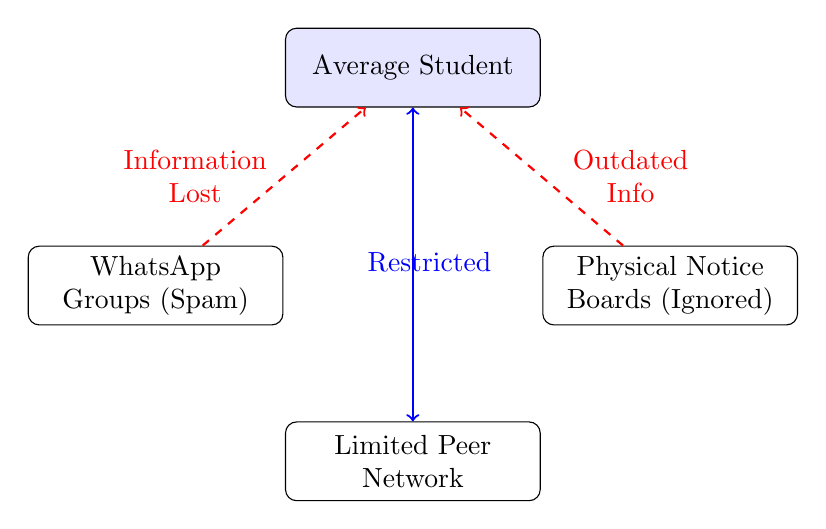
\begin{tikzpicture}[node distance=2.5cm, every node/.style={rectangle, draw, rounded corners, text width=3cm, align=center, minimum height=1cm}]
    % Nodes
    \node (student) [fill=blue!10] {Average Student};
    \node (whatsapp) [below left of=student, xshift=-1.5cm, yshift=-1cm] {WhatsApp Groups (Spam)};
    \node (noticeboard) [below right of=student, xshift=1.5cm, yshift=-1cm] {Physical Notice Boards (Ignored)};
    \node (peers) [below of=student, yshift=-2.5cm] {Limited Peer Network};

    % Arrows
    \draw[->, thick, dashed, red] (whatsapp) -- node[anchor=east, draw=none, text width=2cm, text=red] {Information Lost} (student);
    \draw[->, thick, dashed, red] (noticeboard) -- node[anchor=west, draw=none, text width=2cm, text=red] {Outdated Info} (student);
    \draw[<->, thick, blue] (student) -- node[midway, xshift=6pt, draw=none, text=blue] {\strut Restricted} (peers);
\end{tikzpicture}
\caption{The Fragmented Communication Flow Currently Plaguing the Campus}
\label{fig:silo_diagram}
\end{figure}

\section{Need for Solution}
The campus desperately requires a modern, highly responsive digital ecosystem that permanently bridges the gap between students, resources, and opportunities. A solution is needed that applies strict quality control—such as admin-authorized uploads for PYQs and official event calendars—while simultaneously providing robust, real-time communication tools that do not spam general student groups. This solution must be mobile-first, ensuring every student has the campus in their pocket.